\documentclass[../Kvantemekanik.tex]{subfiles}
 
\begin{document}
\section{Historisk perspektiv}
Historien bag opfindelsen af kvantemekanik er i sig selv utrolig fascinerende og underholdende at læse og høre om. Lige fra hvordan Heisenberg fik idéen til usikkerhedsrelationen i et badekar på loftet af Niels Bohr instituttet, over hvordan Bohr og Einstein glemte at stige af bussen under en ophedet diskussion over guds tilbøjeligheder til hazardspil, til hvordan Schrödinger kom på sin berømte ligning mens han var i et lysthus i de schweiziske alper sammen med en elskerinde (og oprindeligt brugte ligningen som et modargument imod kvantemekanik, da han mente at den gav nogle absurde konsekvenser. Ironisk nok er hans ligning i dag grundlaget  for det hele). Vi vil dog her holde os til de mest essentielle begivenheder, og lade anekdoterne vente til de sene aftener.


Kvantemekanikken beskriver hvordan verden virker på lille skala.
Det betyder blandt andet at vi ikke lægger mærke til kvantefænomener i vores hverdag, og og derfor kan mange kvantefenomener virke uintuitive.
Når man undersøger naturen på lille skala er den dog uundværlig.
Et af de første steder hvor den klassiske fysik var utilstrækkelig er lys.
På Newtons tid var der to modstridende beskrivelser af lyset.
I den ene beskrivelse var lyset strømme af partikler kaldet korpuskler.
I den anden var lyset bølger i et medie kaldet æteren.
Uden eksperimentelt belæg var det ikke muligt at afgøre hvilken model der bedst beskrev virkeligheden.
Det var først i begyndelsen af 1800-tallet at Youngs dobbeltspalteeksperiment viste at lys opførte sig som bølger.
Thomas Young sendte lys igennem to spalter og observerede et interferens mønster på en skærm bagved.
Interferens er et typisk bølgefenomen og ville ikke findes hvis lyset var partikler.
Dette samt Maxwells beskrivelse elektromagnetiske bølger betød at bølgemodellen blev generelt accepteret.
Bølge beskrivelsen havde dog problemer.
Helt grel var beskrivelsen af varmestråling.
Her var det muligt at opstille en model, Rayleigh-Jeans lov, der gav en glimrende beskrivelse ved lange bølgelængder.

$$
B_\lambda (T)= \frac{2c\sub{k}{B}T}{\lambda^4}
$$
Problemet er for korte bølgelængder hvor $\frac{1}{\lambda^4}$ ledert eksploderer, hvilket forudsagde at alle legemer ville udsende uendelige mængder kortbølget lys. Denne såkaldte ultraviolette katastrofe forekommer tydelig vist ikke, da det ikke ville tillade liv som vi kender det i universet.

En tilfredstillende model blev fremstillet af Max Planck, men i hans udregninger antog han at lys kun kunne udsendes i pakker med en energi på:
\begin{equation}
E_\gamma = \frac{h}{\lambda}
\end{equation}
Planck så blot dette som et smart regnetrivk, men i dag ved vi at det var et af de første blik ind i kvantemekanikkens verden. Konstanten $h$ kaldet i dag Plancks konstant og optræder i stort set alle ligninger der involverer kvantemekanik. Ofte bruger man i stedet Plancks reducerede konstant $\frac{h}{2\pi}=\hbar$ ($h$-streg).
Grunden til at kvantemekanikken er ubetydelig i vores hverdag er at Plancks konstant er så uhyre lille. 

\begin{align*}
h &= \SI{6.626e-34}{Js}\\
\hbar &= \SI{1.055e-34}{Js}
\end{align*}

\begin{figure}
    \centering
    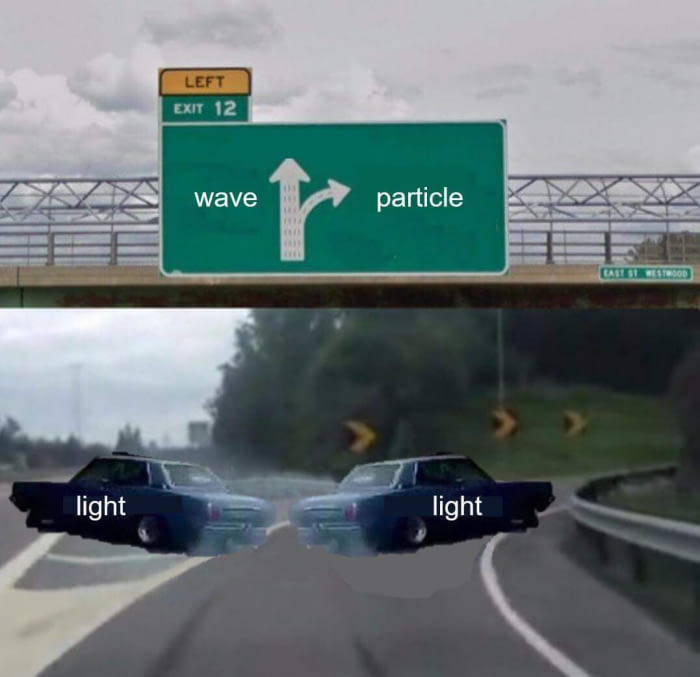
\includegraphics[width = 0.8\textwidth]{Kvantemekanik/billeder/dualitet.jpg}
\end{figure}


At Planck ikke blot havde udført et smart regnetrick fandt man ud af ved at undersøge den fotoelektriske effekt. Hvis man sender ultraviolet lys ind på en metalplade vil lyset slå elektroner fri af metallet, hvilket kan måles. Øger man intensiteten af lyset slår man flere elektroner løs. Hvis man måler de løsrevne elektroners kinetiske energi finder man at der er en øvre grænse for energien. Denne grænse afhænger af lysets bølgelængde.
$$
\sub{T}{max} = \frac{h}{\lambda}-\sub{E}{binding}
$$
Nettop som man ville forvente hvis lyset var kvantiseret. Bølger kommer ikke i diskrete pakker, dette er en klar partikel egenskab.
lige pludselig var partikel modellen ikke helt så død som man havde troet. I 1924 i sin PhD. afhandling fremsatte de Broglie en model hvor ikke kun lys var både var både bølger og partikler, men også alt andet. For ting med masse er bølgelængden bestemt af impulsen(bevægelsesmængden) og dermed hastigheden af partiklen.
\footnote{I de Broglies oprindelige model blev partiklernes bevægelse bestemt af en pilotbølge. Denne fortolkning af kvantemekanikken blev ret hurtigt forkastet. Der er dog en modificeret udgave, de Broglie-Bohm fortolkningen, fra 50'erne.}
\begin{equation}
\lambda = \frac{h}{p} = \frac{h}{mv}
\end{equation}

Året efter opstillede Schrödinger en ligning, der senere er blevet opkaldt efter ham,der beskriver hvordan systemerne udvikler sig over tid. 

\end{document}